\chapter{Aplikace OLS na časové řady}

\section{Stacionární a slabě závislá časová řada}

\subsection{Stacionární a nestacionární časová řada}

\subsubsection{Stacionární stochastický proces}

Stochastický 
proces ${x_t: t = 1, 2, ...}$ je stacionární, jestliže pro 
libovolný výběr časových indexů $1 \le t_1 < t_2 < ... < t_m$ je 
sdružené rozdělení $(x_{t_1}, x_{t_2}, ..., x_{t_m})$ stejné jako 
sdružené rozdělení $(x_{t_1 + h}, x_{t_2 + h}, ..., x_{t_m + h})$ 
pro všechna celá čísla $h \ge 1$.

Zjednodušeně může říci, že 
stacionární časová řada je časová řada, jejíž 
pravděpodobnostní rozdělení je stabilní v čase. 
Pravděpodobnostní rozdělení $x_1$ je tak stejné jako $x_2$ nebo 
$x_3$ - posloupnost $\{x_t; t = 1, 2, ...\}$ sleduje identické 
pravděpodobnostní rozdělení.

Samotná stacionarita však vyžaduje více - např. sdružené 
rozdělení $(x_1, x_2)$ musí být identické se sdruženým 
pravděpodobnostním rozdělením $(x_t, x_{t + 1})$ pro libovolné $t 
\ge 1$. To znamená, že korelace mezi dvěma po sobě jdoucími členy 
časové řady je konstantní napříč celou časovou řadou.

Stochastický proces, který není stacionární, nazýváme 
nestacionárním stochastickým procesem. Příkladem takovéhoto 
procesu je časová řada s trendem, se kterou jsme se setkali v 
minulé kapitole.

\subsubsection{Kovariančně stacionární proces}

Stochastický proces $\{x_t: t = 1, 2, ...\}$ s konečným druhým 
momentem $[E[x_i^2] < \infty]$ je kovariančně stacionární, pokud 
(1) $E[x_t]$ je konstantní, (2) $var[x_t]$ je konstantní a (3) pro 
libovolné $t$ a $h \ge 1$ je $cov[x_t, x_{t + h}]$ pouze funkcí $h$ a 
nikoliv funkcí $t$.

Kovarianční stacionarita se zaměřuje pouze na první dva momenty 
stochastického procesu, kde střední hodnota a rozptyl jsou 
konstantní v čase a kovariance mezi $x_t$ a $x_{t + h}$ závisí 
pouze na jejich vzájemné vzdálenosti $h$.

Jestliže má stacionární proces konečný druhý moment, pak musí 
být kovariančně stacionární. Opačné tvrzení však nemusí být pravdivé.

\subsubsection{Význam stacionarity}

Pokud chceme analyzovat vazby mezi dvěma proměnnými pomocí 
regresní analýzy, musí předpokládat jistou formu jejich stability v 
čase. Jestliže by se vazba mezi těmito dvěma proměnnými (např. mezi $x$ a 
$y$) náhodně měnila s každou časovou periodou, nemohli bychom 
doufat, že této vazbě porozumíme, pokud bychom měli k dispozici 
pouze jednu realizaci podkladového procesu.

\subsection{Slabě závislá časová řada}

Kovariančně stacionární časová 
řada je slabě závislá, pokud korelace mezi $x_t$ a $x_{t + h}$ 
konverguje dostatečně rychle k nule s tím, jak $h \rightarrow \infty$.
Kovariančně stacionární řady, kde $corr[x_t, x_{t+h}] \rightarrow 
0$ pro $h \rightarrow \infty$, nazýváme asymptoticky nekorelované.

Předpoklad slabé závislosti je pro regresní analýzu důležitý, 
protože nahrazuje předpoklad náhodného výběru, který implikuje 
platnost zákona velkých čísel a centrální limitní věty. 
Stacionární slabě závislá časová řada je tak ideální pro 
účely vícerozměrné regresní analýzy.

\subsubsection{Proces klouzavého průměru řádu jedna}

Uvažujme příklad slabě závislé řady
\begin{equation}
x_t = e_t + \alpha_1 e_{t - 1}, ~~~ t = 1, 2, ...,
\end{equation}
kde $\{e_t, t = 0, 1, ...\}$ je nezávislá stejnoměrně rozdělená 
posloupnost s nulovou střední hodnotou a rozptylem $\sigma^2_e$. 
Proces $\{x_t\}$ nazýváme procesem klouzavého průměru řádu jedna 
[moving average process of order one; MA(1)].

Proč je MA(1) proces slabě závislý? Je zřejmé, že po sobě 
jdoucí členy $x_t$ a $x_{t + 1}$ jsou 
korelované. Protože $x_{t + 1} = e_{t + 1} + \alpha_1 e_t$, je 
$cov[x_t, x_{t + 1}]$ rovno $\alpha_1 var[e_t] = \alpha_t \sigma^2_e$. 
A protože $var[x_t] = (1 + \alpha_1^2)\sigma^2_e$, je $corr[x_t, x_{t + 
1}]$ rovno $\frac{\alpha_1}{1 + \alpha_1^2}$. Jakmile se však 
zaměříme na členy posloupnosti, které jsou od sebe dvě a více 
časových period, zjistíme, že jsou nekorelované, protože jsou 
nezávislé. Z důvodu předpokladu nezávislého stejnoměrného 
rozdělení $e_t$ je $\{x_t\}$ stacionární. MA(1) je tak
stacionární slabě závislá posloupností, a proto na ni lze aplikovat 
zákon velkých čísel a centrální limitní větu.

\subsubsection{Autoregresivní proces řádu jedna}

Dalším populárním příkladem stacionární slabě závislé řady 
je tzv. autoregresivní proces řádu jedna [autoregressive process of 
order one; AR(1)].
\begin{equation}
y_t = \rho_1 y_{t - 1} + e_t, ~~~ t = 1, 2, ...
\end{equation}
Počáteční bod řady je $y_0$ a $\{e_t: t = 1, 2, ... \}$ je 
nezávislá stejnoměrně rozdělená posloupnost s nulovou střední 
hodnotou a rozptylem $\sigma^2_e$. Dále předpokládáme, že $e_t$ je 
nezávislé na $y_0$ a že $E[y_0] = 0$.

Klíčovým předpokladem pro slabou závislost AR(1) procesu je tzv. 
podmínka stability $|\rho_1| < 1$. Pak nazýváme $\{y_t\}$ stabilním 
AR(1) procesem.

Předpokládejme, že je výše uvedený proces kovariančně 
stabilní.\footnote{Lze dokázat, že $\{y_t\}$ je striktně 
stacionární. Tento důkaz však přesahuje záběr naší knihy.} 
Tento předpoklad implikuje $E[y_t] = E[y_{t - 1}]$, což pro (11.2) s 
$\rho_1 \ne 1$ může nastat pouze pro $E[y_t] = 0$. Vzhledem k tomu, 
že $e_t$ a $y_{t - 1}$ jsou nezávislé, platí $var[y_t] = \rho_1^2 
\sigma^2_y + \sigma_e^2$. Protože dle podmínky stability platí 
$\rho_1^2 < 1$, získáváme
\begin{equation}
\sigma^2_y = \frac{\sigma_e^2}{1 - \rho_1^2}
\end{equation}

Kovarianci mezi $y_t$ a $y_{t + h}$ pro $h \ge 1$ lze pak odvodit 
následujícím způsobem.
\begin{multline}
y_{t + h} = \rho_1 y_{y + h - 1} + e_{t + h} = \rho_1(\rho_1 y_{t + h - 
2} + e_{t + h -1}) + e_{t + h}\\
= \rho_1^2 y_{t + h - 2} + \rho+1 e_{t + h - 1} + e_{t + h} = ...\\
= \rho_1^h y_t + \rho_1^{h - 1} e_{t + 1} + ... + \rho_1 e_{t + h - 1} 
+ e_{t + h}
\end{multline}
Protože $E[y_t] = 0$, můžeme poslední rovnici vynásobit $y_t$ a 
aplikovat očekávanou hodnotu, abychom získali $cov[y_t, y_{t + h}]$. 
S využitím skutečnosti, že $e_{t + j}$ je nekorelované s $y_t$, 
získáváme
\begin{multline}
  cov[y_t, y_{t + h}]\\
  = E[y_t, y_{t + h}] = \rho_1^h E[y_t^2] + \rho_1^{h 
- 1} E[y_t e_{t + 1}] + ... + E[y_t e_{t + h}]\\
= \rho_1^h E[y_t^2] = \rho^h \sigma_y^2.
\end{multline}
Protože $\sigma_y$ je standardní směrodatná odchylka jak pro $y_t$ 
tak pro $y_{t + h}$, můžeme korelaci mezi $y_t$ a $y_{t + h}$ 
definovat jako
\begin{equation}
corr[y_t, y_{t + h}] = \frac{cov(y_t, y_{t + h})}{\sigma_y \sigma_y} = 
\rho_1^h.
\end{equation}
Korelace dvou po sobě jdoucích členů časové řady je $\rho_1$. Je 
zřejmé, že i když je tato korelace vysoká - řekněme 0.90 - 
korelace mezi $y_t$ a $y_{t + h}$ klesá velmi rychle k nule s tím, 
jak $h \rightarrow \infty$. Proto můžeme AR(1) považovat za slabě 
závislý proces.

Na závěr zdůrazněme, že časová řada sledující trend, 
ačkoliv nestacionární, může být slabě závislá. Časovou řadu, 
která je po odstranění trendu jak stacionární tak slabě 
závislá, nazýváme trendově stacionárním procesem.

\section{Asymptotické vlastnosti OLS}

\begin{assumption}[TS.1' - linearita a slabá závislost]
Uvažujme stejný model jako v případě předpokladu TS.1. Nyní však přidejme předpoklad, že $\{(x_t, y_t): t = 1, 2, ...\}$ je stacionární a slabě závislý proces. V tomto případě lze na výběrové průměry aplikovat zákon velkých čísel a centrální limitní větu.

\raggedleft{$\clubsuit$}
\end{assumption}

Důležitým rozdílem mezi TS.1 a TS.1' je předpoklad slabé závislosti.

\begin{assumption}[TS.2' - neexistence perfektní kolinearity]
Stejný předpoklad jako TS.2.

\raggedleft{$\clubsuit$}
\end{assumption}

\begin{assumption}[TS.3' - nulová podmíněná střední hodnota]
Vysvětlující veličiny $x_t = (x_{t1}, x_{t2}, ..., x_{tj})$ jsou souběžně exogenní tak, jak je tomu v rovnici (10.16), tj. $E[u_t|x_t] = 0$.
  
\raggedleft{$\clubsuit$}
\end{assumption}

TS.3' je mnohem méně restriktivní než TS.3, protože TS.3' neklade žádná omezení na to, jaký má být vztah mezi $u_t$ a vysvětlujícími veličinami v ostatních časových periodách. Nicméně stacionarita implikuje, že pokud souběžná exogenita platí pro jednu časovou periodu, pak platí pro všechny časové periody. Pokud bychom se zbavili předpokladu stacionarity, museli bychom požadovat splnění TS.3' pro všechny časové periody $t = 1, 2, ...$.

Předpoklad konzistentnosti OLS, který je představen ve větě 11.1, pouze vyžaduje, aby $u_t$ mělo nulovou nepodmíněnou střední hodnotu a bylo nekorelované s libovolným $x_{ij}$, tj.
\begin{equation}
E[u_t] = 0, ~~~ cov[x_{tj}, u_t] = 0, ~~~ j = 1, 2, ..., k.
\end{equation}

V následujícím textu budeme převážně pracovat s předpokladem nulové podmíněné střední hodnoty, protože vede k nejpřímější definici asymptotické analýzy.

\begin{theorem}[Konzistentnost OLS]
Při splnění předpokladů TS.1', TS.2' a TS.3' jsou OLS odhady konzistentní, tj. $plim \hat{\beta}_j = \beta_j$ pro $j = 0, 1, ..., k$.
  
\raggedleft{$\clubsuit$}
\end{theorem}

Mezi větami 10.1 a 11.1 existuje několik praktických odlišností. Za prvé, ve větě 11.1 jsme došli k závěru, že OLS odhady jsou konzistentní. Tato věta nám však neříká nic o jejich nestrannosti. Za druhé, ve větě 11.1 jsme na jedné straně oslabili význam, ve kterém musí být vysvětlující veličiny exogenní, na druhé straně avšak musí být podkladová časová řada slabě závislá. Slabá závislost je klíčová pro získání distribucí odhadů regresních parametrů; tomuto tématu se budeme věnovat v následující kapitole.

Pro ilustraci uvažujme AR(1) proces
\begin{equation}
y_t = \beta_0 + \beta_1 y_{t - 1} + u_t,
\end{equation}
kde
\begin{equation}
E[u_t | y_{t - 1}, y_{t - 2}, ...] = 0.
\end{equation}
Pokud spojíme tyto dvě rovnice, získáme
\begin{equation}
E[y_t | y_{t - 1}, y_{t - 2}, ...] = E[y_t | y_{t - 1}] = \beta_0 + \beta_1 y_{t - 1}.
\end{equation}

Protože v roli vysvětlující veličiny vystupuje pouze $y_{t-1}$, implikuje (11.9) platnost předpokladu TS.3'. Předpoklad striktní exogenity, tj. předpoklad TS.3, který je nezbytný pro nezkreslenost OLS odhadů, splněn není. V AR(1) procesu vysvětlující veličiny obsahují všechny hodnoty $y$ s výjimkou té poslední, tj. $(y_0, y_1, ..., y_{n - 1})$. Předpoklad TS.3 však vyžaduje, aby pro všechna $t$ bylo $u_t$ nekorelováno s $y_0, y_1, ..., y_{n - 1}$, což zcela zřejmě není splněno. Navíc, protože $E[u_t] = 0$ a $corr[y_{t - 1}, u_t] = 0$, musí být $u_t$ a $y_t$ korelováno.
\begin{multline}
cov[y_t, u_t] = E[y_t, u_t] - E[y_t]E[u_t] = E[y_t, u_t]\\
= E[(\beta_0 + \beta_1 y_{t - 1} + u_t)u_t] = \beta_0 E[u_t] + \beta_1 E[y_{t - 1} u_t] + E[u^2_t]\\
= E[u^2_t] = E[u^2_t] - E[u_t]^2 = var[u_t] > 0  
\end{multline}
Je tedy zřejmé, že AR(1) nemůže splňovat předpoklad TS.3.

Pro splnění předpokladu slabé závislosti musí být $|\beta_1| < 1$. Jestliže je tento předpoklad splněn, pak věta 11.1 implikuje, že OLS odhady jsou konzistentní. Bohužel $\hat{\beta}_1$ není nestranný a míra zkreslení může být značná, pokud se jedná o vzorek malého rozsahu nebo pokud je $\beta_1$ blízké jedné.\footnote{Pro $\beta_1$ blízké jedné může $\hat{\beta}_1$ výrazně podhodnocovat skutečnou hodnotu $\beta_1$.} Pro vzorky středního nebo velkého rozsahu by $\hat{\beta}_1$ mělo být dobrým odhadem $\beta_1$.

\begin{assumption}[TS.4' - homoskedasticita]
Chyby regresního modelu jsou souběžně homoskedasticitní, tj. $var[u_t | x_t] = \sigma^2$.

\raggedleft{$\clubsuit$}
\end{assumption}

\begin{assumption}[TS.5' - neexistence autokorelace]
Pro všechna $t \ne s$ platí $E[u_tu_s|x_t, x_s] = 0$.

\raggedleft{$\clubsuit$}
\end{assumption}

Všimněme si, že v TS.4' na rozdíl od TS.4 podmiňujeme pouze na vysvětlující veličiny v čase $t$. V TS.5' pak podmiňujeme pouze na vysvětlující veličiny v časových periodách, které se shodují s $u_t$ a $u_s$. V praxi však velice často ignorujeme podmínění na $x_t$ a $x_s$ a namísto toho uvažujeme, že $u_t$ a $u_s$ jsou nepodmíněně nekorelované pro všechna $t \ne s$.

Autokorelace je častý problém statických modelů a modelů s konečným rozdělením zpoždění - neexistuje nic, co by garantovalo neexistenci korelace $u_t$ v čase. Nicméně TS.5' platí pro AR(1) proces tak, jak je formulován v (11.8) a (11.9). Protože vysvětlující veličina v čase $t$ je $y_{t - 1}$, musíme dokázat, že $E[u_t u_s | y_{t - 1} y_{s - 1}] = 0$ pro všechna $t \ne s$. Pro ilustraci uvažujme $s < t$.\footnote{Na opačný případ lze aplikovat princip symetrie.} Protože $u_s = y_s - \beta_0 - \beta_1 y_{s - 1}$, je $u_s$ funkcí $y$ před časem $t$. Dle (11.9) platí $E[u_t|u_s, y_{t - 1}, y_{s - 1}] = 0$, a proto $E[u_t u_s| u_s, y_{t - 1}, y_{s - 1}] = u_s E[u_t | y_{t - 1}, y_{s - 1}] = 0$. Zákon iterované střední hodnoty (law of iterated expectations) implikuje $E[u_t s_t | y_{t - 1}, y_{s - 1}] = 0$. Toto je velmi důležitý závěr - pokud (11.8) obsahuje pouze jedno zpoždění, nejsou chyby regresního modelu autokorelované.

\begin{theorem}[Asymptotická normalita OLS odhadů]
Při splnění předpokladů TS.1' až TS.5' sledují OLS odhady asymptoticky normální rozdělení. Také klasické $t$ a $F$ statistiky jsou asymptoticky platné.
  
\raggedleft{$\clubsuit$}
\end{theorem}

Výše uvedená věta tedy říká, že i když nejsou předpoklady klasického lineárního modelu bez zbytku splněny, jsou OLS odhady konzistentní a lze použít obvyklé procedury pro jejich odhad a to včetně stanovení intervalů spolehlivosti.

Při splnění předpokladů TS.1' až TS.5' lze dokázat, že OLS odhady jsou asymptoticky efektivní v rámci rodiny odhadů popsaných ve větě 5.3.\footnote{Pouze nahradíme index náhodného výběru $i$ časovým indexem $t$.} Také modely, které zahrnují trend, mohou splňovat požadavky TS.1' až TS.5' za předpokladu, že jsou trendově stacionární. Pokud je časový trend explicitně zahrnut do regresního modelu, lze také použít obvyklé postupy pro odhad parametrů.

\section{Persistentní časové řady v regresní analýze}

V praxi se poměrně často setkáváme s časovými řadami, které nesplňují podmínku slabé závislosti. Aplikace regresní analýzy na časové řady, které vykazují silnou závislost v čase, nepředstavuje zásadní problém, pokud jsou splněny CLM předpoklady, které jsme představili v kapitole 10. Nicméně stanovení intervalů spolehlivosti jednotlivých odhadů může být značně zavádějící, protože se již nelze spolehnout na zákon velých čísel a centrální limitní větu.

\subsection{Persistentní časové řady}

AR(1) proces je slabě závislý, pokud $|\rho_1| < 1$. Nicméně v praxi mnoho časových řad lépe charakterizuje model
\begin{equation}
y_t = y_{t - 1} + e_t, ~~~ t = 1, 2, ...,
\end{equation}
kde $\{e_t: t = 1, 2, ...\}$ sleduje nezávislé identické pravděpodobnostní rozdělení s nulovou střední hodnotou a rozptylem $\sigma^2$. Tento proces nazýváme náhodnou procházkou. Předpokládejme, že $y_0$ je nezávislé na $e_t$ pro všechna $t \ge 1$. Pak lze střední hodnotu $t_t$ snadno určit pomocí opakované substituce
\begin{equation}
y_t = e_t + e_{t - 1} + ... + e_1 + y_0
\end{equation}
a následnou aplikací očekávané hodnoty
\begin{equation}
E[y_t] = E[e_t] + E[e_{t - 1}] + ... + E[e_1] + E[y_0] = E[y_0].
\end{equation}
Očekávaná hodnota náhodné procházky je tak nezávislá na čase $t$. Obvyklý předpoklad je $y_0 = 0$, což implikuje $E[y_t] = 0$ pro všechna $t$.

Naproti tomu rozptyl náhodné procházky narůstá s časem $t$, a proto se nejedná o stacionární proces. Předpokládejme, že $y_0$ je nenáhodné, tj. $var[y_0] = 0$. Protože $\{e_t\}$ sleduje identické nezávislé rozdělení, platí
\begin{equation}
var[y_t] = var[e_t] + var[e_{t - 1}] + ... + var[e_t] = \sigma_e^2 t.
\end{equation}
Navíc náhodná procházka vykazuje značně persistentní chování, což znamená, že hodnota $y$ dnes je důležitá pro určení hodnoty $y$ i ve velmi vzdálené budoucnosti. Pro ilustraci rozepišme $h$ časových period jako
\begin{equation}
y_{t + h} = e_{t + h} + e_{t + h - 1} + ... + e_{t + 1} + y_t.
\end{equation}
Předpokládejme, že chceme vypočíst očekávanou hodnotu $y_{t + h}$ pro danou hodnotu $y_t$. Z výše uvedené rovnice je zřejmé, že
\begin{equation}
E[y_{t + h}|y_t] = y_t.
\end{equation}
Jinými slovy, nejlepším odhadem budoucí hodnoty $y_{t + h}$ je současná hodnota $y_t$ a to bez ohledu na to, jak vzdálenou budoucnost uvažujeme. To lze postavit do kontrastu se stabilním AR(1) procesem, kde byl podobný postup použit jako důkaz pro
\begin{equation}
E[y_{t + h} | y_t] = \rho_1^h y_t,
\end{equation}
kde $E[y_{t + h}|y_t]$ se blíží nepodmíněné střední hodnotě $E[y_t] = 0$ s tím, jak $h \rightarrow \infty$, a to bez ohledu na hodnotu $y_t$.

Lze dokázat, že v případě náhodné procházky $\{y_t\}$ se korelace mezi $y_t$ a $y_{t + h}$ pro dostatečně velké $t$ blíží jedné. Za předpokladu $var[y_0] = 0$ totiž platí
\begin{equation}
corr[y_t, y_{t + h}] = \sqrt{\frac{t}{t + h}}.
\end{equation}
Korelace tak závisí na počátečním bodu $t$, a proto $\{y_t\}$ není kovariančně stacionární. Ačkoliv pro fixní $t$ se korelace blíží nule s tím, jak se $h$ blíží nekonečnu, není tato konvergence dostatečně ``rychlá''.  Pro libovolné $h$ lze vždy zvolit $t$ dostatečně vysoké na to, aby se $corr[y_t, y_{t + h}]$ blížilo jedné. Náhodná procházka tak nesplňuje požadavek na asymptoticky nekorelovanou řadu.

Jak nározně ilustruje následující graf, je v praxi velmi obtížné vizuálně rozlišit, zda-li je daný proces náhodnou procházkou či nikoliv.
\begin{figure}[htp]
\centering
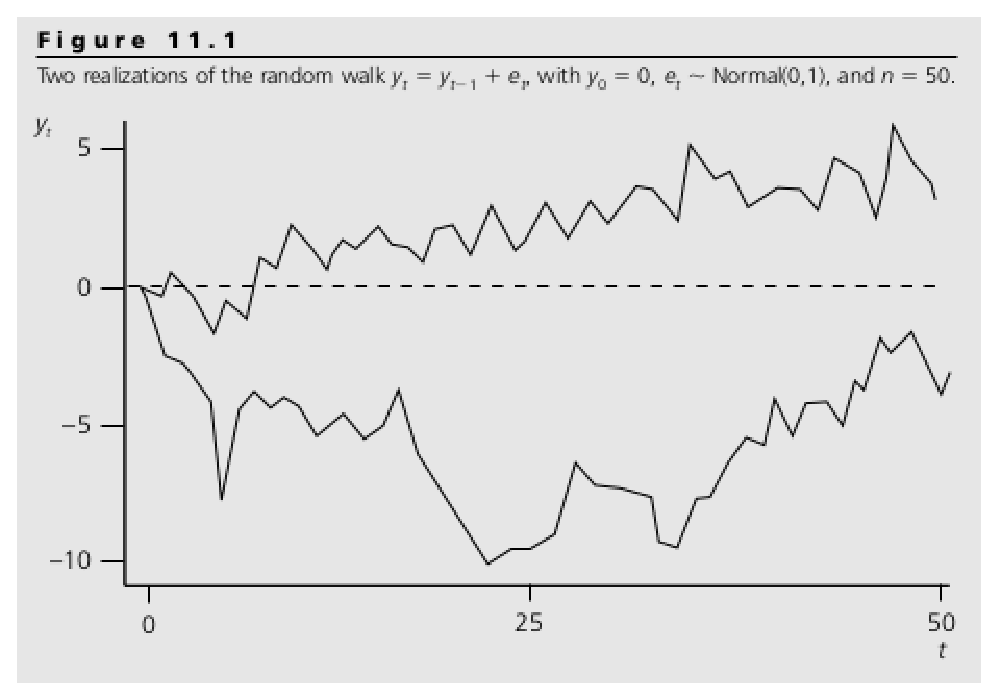
\includegraphics[scale = 0.5]{pictures/figure_11_1.eps}
\caption{Dvě náhodné procházky}
\label{figure_11_1}
\end{figure}
Náhodná procházka je specifickým příkladem tzv. procesu s jednotkovým kořenem (unit root process). Jméno procesu vychází ze skutečnosti, že se jedná o AR(1) model s $\rho_1 = 1$.

Je velmi důležité nezaměňovat časový trend s persistentním charakterem časové řady. Časová řada muže sledovat trend a přitom nebýt persistentní. Existuje však také řady, které jsou persitentní a přitom nesledují žádný trend - příkladem takové řady může být (alespoň pro určitá období) vývoj nezaměstnanosti či inflace. Velice často se však můžeme setkat s řadami, které jsou persistentní a navíc sledující trend. Triviálním příkladem takovéto řady je náhodná procházka s trendem
\begin{equation}
y_t = \alpha_0  + y_{t - 1} + e_t, ~~~ t = 1, 2, ...,
\end{equation}
kde $\{e_t: t = 1, 2, ...\}$ a $y_0$ splňují stejné podmínky jako v případě klasické náhodné procházky. Nově přibyl parametr $\alpha$, který představuje časový trend. S použitím opakované substituce lze snadno dokázat, že střední hodnota tohoto procesu je funkcí času.
\begin{multline}
  E[y_t] = E[\alpha_0t + e_t + e_{t - 1} + ... + e_t + y_0] = \alpha_0 t + E[e_t]\\
  + E[e_{t - 1}] + ... + E[e_1] + E[y_0] = \alpha_0 t
\end{multline}
Podobně jako v případě klasické náhodné procházky lze také v případě náhodná procházky s trendem dokázat, že $E[y_{t + h}|y_t] = a_0 h + y_t$. Rozptyl $y_t$ je stejný jako v případě obyčejné náhodné procházky.

Následující graf zobrazuje náhodnou procházku s trendem. Je zřejmé, že proces sleduje lineární časový trend, nicméně nemá tendenci se vracet k trendové linii.
\begin{figure}[htp]
\centering
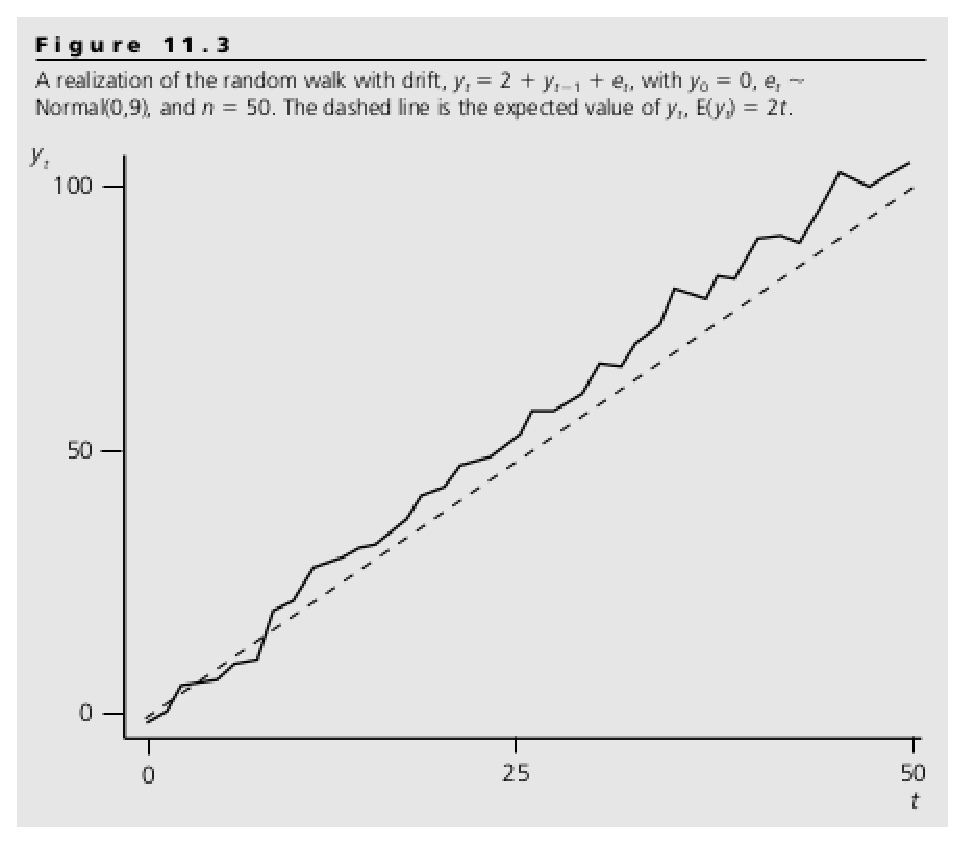
\includegraphics[scale = 0.5]{pictures/figure_11_2.eps}
\caption{Náhodná procházka s trendem}
\label{figure_11_2}
\end{figure}

Náhodná procházka s trendem je příkladem procesu s jednotkovým kořenem, protože se zjevně jedná o AR(1) s  $\rho_1 = 1$.
\begin{equation}
y_t = \alpha_0 + \rho_1 y_{t - 1} + e_t
\end{equation}

\subsubsection{Transformace persistentních časových řad}

Aplikace regresního modelu na časové řady s jednotkovým kořenem může vést k zavádějícím závěrům, pokud jsou porušeny CLM předpoklady.

O slabých závislých časových řadách říkáme, že jsou integrované stupněm nula (integrated of order zero) a značíme je jako $I(0)$. Na tyto časové řady může být aplikována regresní analýza. Procesy s jednotkovým kořenem jako je náhodná procházka (jak s trendem tak bez něj) jsou integrovány stupněm jedna a značíme je jako $I(1)$. Na takovouto časovou řadu musíme nejprve aplikovat diferenci prvního řádu, čímž získáme $I(0)$, a teprve po té ji můžeme použít jako vstup pro regresní analýzu.

Koncept $I(1)$ procesu se nejsnáze vysvětluje na náhodné procházce. Pro $y_t$ generované dle (11.12) totiž platí
\begin{equation}
\Delta y_t = y_t -  y_{t - 1} = e_t, ~~~ t = 2, 3, ...,
\end{equation}
takže $\{\Delta y_t: t = 2, 3, ...\}$ představuje identickou nezávisle rozdělenou posloupnost a je tak slabě závislé. Aplikace diference prvního řádu má však další výhodu a tou je odstranění případného lineárního časového trendu.

\subsubsection{Testování $I(1)$ procesu}

Rozhodování o tom, zda-li je realizace určité časové řady procesem s jednotkovým kořenem, je poměrně komplikované. Tématu se budeme do hloubky zabývat v kapitole 18.

Velmi jednoduchý test je založen na AR(1) modelu - proces je $I(0)$ pokud $|\rho_1| < 1$ a $I(1)$ pokud $\rho_1 = 1$. V předchozím textu jsme prokázali, že pokud je $AR(1)$ proces stabilní, pak $\rho_1 = corr[y_t, y_{t - 1}]$. Proto lze $\rho_1$ odhadnout pomocí výběrové korelace mezi $y_t$ a $y_{t - 1}$. Tuto výběrovou korelaci nazýváme autokorelací prvního řádu a značíme ji jako $\hat{\rho}_1$. S využitím zákona velkých čísel lze dokázat, že $\hat{\rho}_1$ je při splnění podmínky $|\rho_1| < 1$ konzistentním odhadem $\rho_1$.\footnote{Nicméně $\hat{\rho}_1$ není nezkresleným odhadem $\rho_1$.}

Hodnotu $\hat{\rho}_1$ pak lze použít při rozhodování o tom, zda-li je určitý proces $I(0)$ nebo $I(1)$. Teoreticky by mělo stačit určit konfidenční interval pro $\rho_1$ a zkontrolovat, zda-li obsahuje hodnotu $\rho_1 = 1$. Bohužel výběrová distribuce funkce odhadu $\hat{\rho}_1$ je extrémně odlišná populační distribuce, pokud je $\rho_1$ blízké jedné nebo výrazně menší než jedna. Prozatím tedy budeme použít $\hat{\rho}_1$ jako přibližný indikátor toho, zda-li máme na časovou řadu aplikovat diferenci prvního řádu.

Jestliže časová řada vykazuje silný trend, je vhodné aplikovat diferenci prvního řádu až po odstranění trendu. Jestliže z časové řady není odstraněn trend, pak je autoregresivní korelace výrazně nadhodnocená, což zvyšuje ``pravděpodobnost'' indikace jednotkového kořene.  

\subsection{Dynamicky kompletní modely a absence autokorelace}

Uvažujme následující jednoduchý regresní model
\begin{equation}
y_t = \beta_0 + \beta_1 z_t + u_t.
\end{equation}
Pro konzistenci OLS odhadů postačuje, pokud $E[u_t | z_t] = 0$. Obecně platí, že $\{u_t\}$ může být autokorelované. Nicméně, pokud předpokládáme
\begin{equation}
E[u_t|z_t, y_{t - 1}, z_{t - 1}, ...] = 0,
\end{equation}
pak, jak si ukážeme později, je předpoklad TS.5' splněn. Konkrétně $\{u_t\}$ není autokorelované. Rovnice (11.25) implikuje souběžnou exogenitu $z_t$, tj. $E[u_t|z_t] = 0$.

Abychom získali lepší vhled do problému, aplikujme podmíněné očekávání na (11.24) a použijme (11.25), čímž získáme
\begin{equation}
E[y_t|z_t, y_{t - 1}, z_{t - 1}, ...] = E[y_t | z_t] = \beta_0 + \beta_1 z_t + E[u_t|z_t] = \beta_0 + \beta_1 z_t.
\end{equation}
Tato rovnice nám říká, že v okamžiku fixace $z_t$ nejsou zpožděná $y$ a $z$ schopna vysvětlit aktuální hodnotu $y$. Pokud tento předpoklad není splněn, pak je $\{u_t\}$ autokorelované.

Dále uvažujme model se dvěma zpožděními.
\begin{equation}
y_t = \beta_0 + \beta_1 z_t + \beta_2 z_{t - 1} + \beta_3 z_{t - 2} + u_t
\end{equation}
Vzhledem k definici modelu má podmíněná střední hodnota tvar
\begin{equation}
E[y_t | z_t, z_{t - 1}, z_{t - 2}, z_{t - 3}, ...] = E[y_t | z_t, z_{t - 1}, z_{t - 2}].
\end{equation}
Podobně jako předchozím případě pak předpokládáme, že po fixaci $z_t$, $z_{t - 1}$ a $z_{t - 2}$ nemá žádné zpožděné $y$ a žádné $z$ se zpožděním větším než dva schopnost vysvětlit aktuální hodnotu $y$, tj.
\begin{equation}
E[y_t| z_t, y_{t - 1}, z_{t - 1}, ...] = E[y_t | z_t, z_{t - 1}, z_{t - 2}].
\end{equation}

Nakonec uvažujme obecný model
\begin{equation}
y_t = \beta_0 + \beta_1 x_{t1} + ... + \beta_k x_{tk} + u_t,
\end{equation}
kde vysvětlující veličiny $x_t = (x_{t1}, ..., x_{tk})$ mohou zahrnovat jak zpožděná $z$, tak zpožděná $y$. Rovnice (11.25) tak přejde do tvaru
\begin{equation}
E[u_t|x_t, y_{t - 1}, x_{t - 1}, ...] = 0,
\end{equation}
což vyjádřeno pomocí $y_t$ znamená
\begin{equation}
E[y_t | x_t, y_{t - 1}, x_{t - 1}, ...] = E[y_t | x_t].
\end{equation}
Jinými slovy, do matice $x_t$ byl zařazen dostatek zpožděných veličin tak, aby další zpožděné $y$ a další zpožděné vysvětlující veličiny $z$ měly ve vztahu k aktuální hodnotě $y$ nulovou vypovídající hodnotu. Takovýto model nazýváme dynamicky kompletním modelem. Protože (11.31) je ekvivalentní
\begin{equation}
E[u_t | x_t, u_{t - 1}, x_{t - 1}, u_{t - 2}, ...] = 0,
\end{equation}
lze dokázat, že dynamicky kompletní model splňuje předpoklad TS.5'. Pro ilustraci uvažujme $s < t$; s využitím zákona o iterované střední hodnotě pak získáme
\begin{multline}
  E[u_tu_s|x_t,x_s] = E\big[E[u_t u_s|x_t, x_s, u_s]|x_t, x_s\big]\\
  = E\big[u_sE[u_t|x_t, x_s, u_s]|x_t, x_s\big].
\end{multline}
Protože $s < t$, je $(x_t, x_s, u_s)$ podmnožinou podmínění v rovnici (11.33), což implikuje $E[u_t|x_t, x_s, u_s] = 0$. To znamená, že
\begin{equation}
E[u_t u_s | x_t, x_s] = E[u_s \cdot 0 | x_t, x_s] = 0,
\end{equation}
a proto je předpoklad TS.5' splněn. Vzhledem k tomu, že dynamicky kompletní model znamená neexistenci autokorelace chybového členu regresního modelu, měly by ideálně všechny modely být dynamicky kompletní.

Pojem dynamická kompletnost by neměl být zaměňován se slabším předpokladem zahrnutí vhodných zpoždění do regresního modelu. V případě modelu (11.30) jsou vysvětlující veličiny $x_t$ sekvenčně exogenní (sequentially exogenous), jestliže
\begin{equation}
E[u_t| x_t, x_{t - 1}, ...] = E[u_t] = 0, ~~~ t = 1, 2, ...
\end{equation}
Je důležité si uvědomit, že striktní exogenita implikuje sekvenční exogenitu, která implikuje souběžnou exogenitu. Protože $(x_t, x_{t - 1}, ...)$ je podmnožinou $(x_t, y_{t - 1}, x_{t - 1}, ...)$, je sekvenční exogenita implikována dynamickou kompletností.

\subsection{Předpoklad homoskedasticity}

V rámci jednoduchého modelu
\begin{equation}
y_t = \beta_0 + \beta_1 z_t + u_t
\end{equation}
vyžaduje předpoklad TS.4', aby
\begin{equation}
var[u_t|z_t] = \sigma^2.
\end{equation}
Ačkoliv je tedy $E[y_t|z_t]$ lineární funkcí $z_t$, musí být $var[y_t|z_t]$ konstantní.

V případě AR(1) procesu má předpoklad homoskedasticity formu
\begin{equation}
var[u_t | y_{t - 1}] = var[y_t | y_{t - 1}] = \sigma^2.
\end{equation}

V případě modelu
\begin{equation}
y_t = \beta_0 + \beta_1 z_t + \beta_2 y_{t - 1} + \beta_3 z_{t - 1} + u_t
\end{equation}
má pak předpoklad homoskedasticity tvar
\begin{equation}
var[u_t | z_t, y_{t - 1}, z_{t - 1}] = var[y_t|z_t, y_{t - 1}, z_{t - 1}] = \sigma^2.
\end{equation}

Obecně tedy platí, že bez ohledu na to, jaká vysvětlující veličina se objeví v regresním modelu, musí být splněn předpoklad, že rozptyl $u_t$ (a tím pádem také $y_t$) je po zafixování těchto veličin konstantní.
